\chapter{Background}

\section{A Brief Introduction to Reservoir Computing}

Recurrent Neural Networks, as opposed to feed-forward neural networks,
are notoriously time consuming and difficult to \cm{train}.
This is \cm{due to} feedback from the recurrent connections during the training process,
allowing small topology changes to drastically change a network's position in the fitness landscape.

It was therefore proposed both in \cite{jaeger2002adaptive} (as Echo State Networks, or ESN)
and \cite{natschlager2002liquid} (as Liquid State Machines, or LSM) to separate the RNN into two parts,
the untrained reccurrent reservoir, and the trained readout layer.
Both of these methods have been unified into the field of Reservoir Computing,
now focusing on the separate training and evolution of the recurrent and readout parts \cite{lukovsevivcius2012reservoir}.

Exiting applications of Reservoir Computing include speech and handwriting recognition,
as well as controlling robotics \cite{lukovsevivcius2012reservoir}.

\section{Alternatives to classical reservoirs}

Are there other types of complex systems that can be used as reservoirs?
What properties must these reservoirs have to be able to solve problems?

Complex networks similar to the sparsely connected RNNs used  ESN and LSM systems include Cellular Automata and Random Boolean Networks.

Cellular Automata are regular grids of cells containing some state,
each cell connected to its neighbors in the grid.
Cells then update in lockstep according to some shared transition table,
creating a new generation.
RBNs can be seen upon as an abstraction over CAs again,
allowing for nonlocal neighbors, and will be introduced in depth in \ref{section:rbns}.

Both models are simple, and can be implemented in software,
hardware (FPGAs), and in materio \cite{miller2002evolution}
(for evolving CAs in materio, see \cite{farstad2015evolving}).
This computational paradigm is known as Cellular Computing,
and provides a potentially powerful alternative to classical computers,
leveraging extreme parallelism, simple components and local state \cite{sipper1999emergence}.

The 'Water bucket' paper investigated the use of an actual bucket of water as a reservoir \cite{fernando2003pattern},
successfully recognizing patterns and achieving decent performance at that.
The RBN Reservoir approach has also been found to be viable \cite{rbn-reservoir} .

\section{A Brief Introduction to Boolean Networks}
\label{section:rbns}

Random Boolean Networks, also known as Kaffman networks,
were originally developed as a model of gene regulatory networks \cite{kauffman1969metabolic},
the complex system that regulates how genes in multicellular organisms interact with each other.
The model requires no assumptions about the inner workings of the actual nodes,
which allows it to model phenomena where the exact internal workings of the system may be unknown.

The simplification of a system to a boolean model doesn't pose a problem,
as any multi-valued network can be transformed to a corresponding binary one.

A RBN is usually described by its number of nodes $N$ and the in-degree $K$ of the nodes,
that is, how many nodes each node depends on (also known as its ancestors).
RBNs can have both homogenous and heterogenous in-degrees.
In heterogenous networks, one usually describes the average connectivity $\langle K \rangle$ instead.

Each node can have a state of zero or one.
The next state of the node is solely determined by the current combination of states of its ancestors.
Each combination leads to a new state of zero or one,
with the probability given by a binomial distribution usually having $\langle P \rangle = 0.5$.
Figure \ref{figure:sample-homogenous-rbn} visualizes a homogenous RBN with $N=3, K=2, P=0.5$.

\begin{figure}
  \centering
  \subfloat[RBN topology]{
    \begin{tikzpicture}[node distance = 5em]
      \node[vertex] (a) {a};
      \node[vertex] (b) [below left of=a] {b};
      \node[vertex] (c) [below right of=a] {c};

      \draw[edge] (a) to[bend right] (b);
      \draw[edge] (a) to (c);

      \draw[edge] (b) to (a);
      \draw[edge] (b) to[bend right] (c);

      \draw[edge] (c) to[bend right] (a);
      \draw[edge] (c) to (b);
    \end{tikzpicture}
  }
  \subfloat[Transition table for node a]{
    \begin{tabular}[b]{ c c | c}
      \multicolumn{2}{c}{Ancestor states} & New state \\
      \hline
      0 & 0 & 0 \\
      0 & 1 & 1 \\
      1 & 0 & 0 \\
      1 & 1 & 1 \\
    \end{tabular}
  }
  \caption{An example homogenous RBN with $N=3, K=2, P=0.5$.}
  \label{figure:sample-homogenous-rbn}
\end{figure}

In the simplest RBN updating scheme, all nodes update in lockstep.
This is known as the Classical RBN updating scheme (CRBN).
The states of the RBN at the next timestep $t+1$ therefore only depend on the states at the previous timestep $t$.
A criticism of the classical model is that gene regulation networks are updating continiously,
as opposed to in lockstep.c
There are therefore a number of alternate updating schemes which can be categorized by whether they are deterministic or nondeterministic, as well as synchronous and asynchronous.

The dynamics of an RBN can be categorized as being in either the ordered, critical, or chaotic phase.
These phases can be identified by how large a part of the network state is able to change over time,
whether similar states tend to converge or diverge over time,
and the networks resistance to perturbations (outside changes to the network).

One way to obtain these phases analytically is by comparing the resulting states of two identical RBNs where one is subject to some perturbation \cite{gershenson2004introduction}.
For visual identification, we plot the states of the RBN in a square lattice,
with the network states plotted horizontally, and time flowing downwards.
A node is drawn as white if its state is one, black otherwise.
The phases are visualized in Figure \ref{figure:rbn-phases}.

\begin{figure}
  \subfloat[Ordered phase, K=1]{
    
\includegraphics[width=0.3\columnwidth]{background/ordered-phase.pdf}
    \label{figure:rbn-ordered}
  }
  \subfloat[Critical phase, K=2]{
    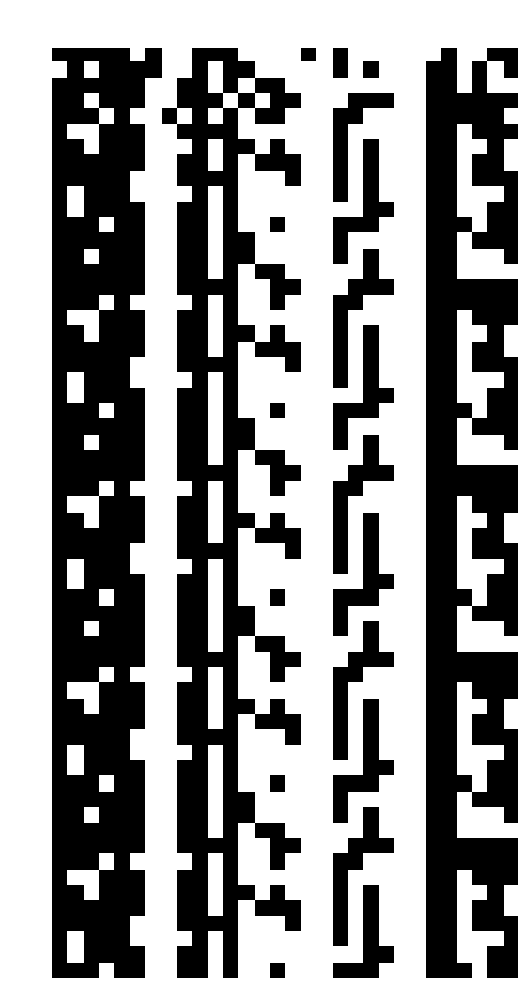
\includegraphics[width=0.3\columnwidth]{background/critical-phase.pdf}
    \label{figure:rbn-critical}
  }
  \subfloat[Chaotic phase, K=3]{
    
\includegraphics[width=0.3\columnwidth]{background/chaotic-phase.pdf}
    \label{figure:rbn-chaotic}
  }

  \caption{
    Trajectories through state-space for RBNs with $N=30, K=[1,2,3]$, visualizing the different phases.
    Time flows downwards the lattice, while RBN states are shown along the X-axis.
    with the network states plotted horizontally, and time flowing downwards.
    Images created with the developed RBN-simulator.
  }
  \label{figure:rbn-phases}
\end{figure}

In general, RBNs in the critical phase are the most interesting.
These are seemingly able to support information transmission, storage and modification,
all capacities required for computation \cite{langton3computation}.
Critical systems are found on the edge of chaos,
on the phase transition between ordered and chaotic networks \cite{gershenson2004introduction}.
For RBNs with $\langle p \rangle = 0.5$,
critical dynamics are usually found at $\langle K \rangle = 2$ \cite{gershenson2004introduction},
although one could still find networks with such dynamics for different values of $\langle K \rangle$.

A thorough introduction to the field of RBNs is available in \cite{gershenson2004introduction}.

\section{RBN Reservoir systems}
\label{subsection:rbn-reservoir-systems}

How does one adapt a RBN for use as a reservoir in a RBN-RC device?
RBNs aren't usually designed to take external input.
We do however, have the concept of perturbation,
the external flipping of bits in the network's state,
transition tables or edges.
This can be utilized to create RBNs that take input,
by continiously perturbing the RBN nodes by the bits of the input sequence.

Questions that follow are how many bits should the network consume at a time,
how many of the network nodes should be perturbed by the input at each timestep,
and what dynamics must such a reservoir have to allow for the computation of interesting problems?

\subsection{A working system}

In \cite{rbn-reservoir} the authors create and analyze functioning RBN-RC systems.
These RBN-RC systems have heterogenous connectivity,
consume one bit of input at each timestep ($I=1$),
perturbing $L$ of the $N$ nodes in the process.
The readout layer can be any node performing some kind of regression of the reservoir state against expected outout for the current task, e.g. linear regression.
Such a setup is shown in Figure \ref{figure:rbn-reservoir}.

\begin{figure}
  \centering
  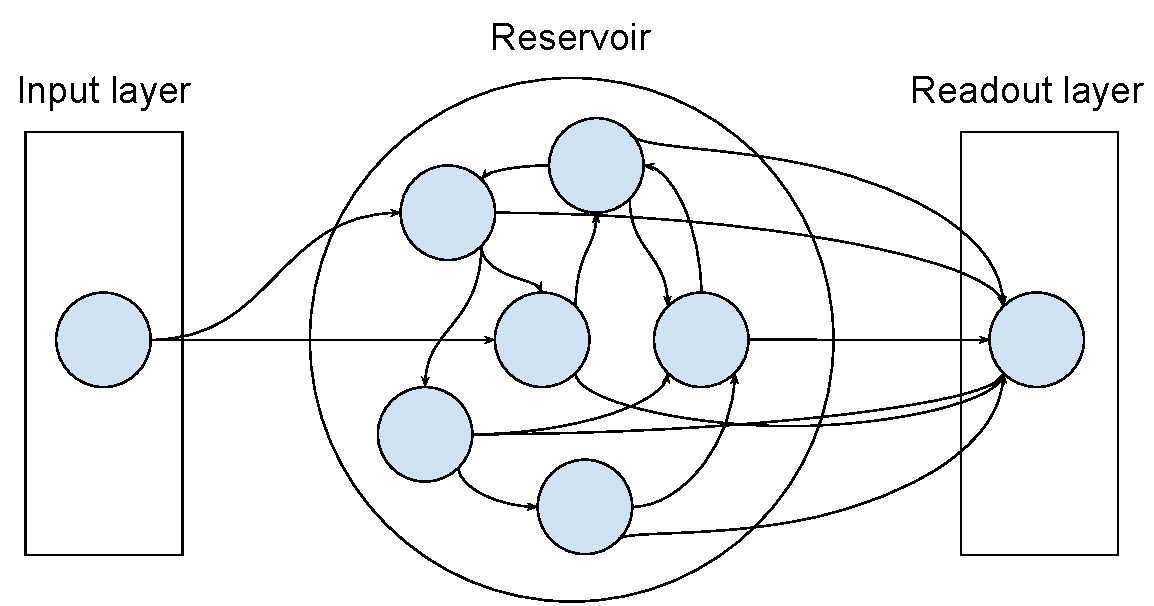
\includegraphics[width=\columnwidth]{background/RBN-Reservoir.pdf}
  \caption{
    RBN-Reservoir system with $I=1, L=2, K=2, N=5$.
    The reservoir transforms the problem from a temporal one to a multidimentional spatial one.
    The readout layer the performs some kind of learning on the reservoir states against the expected output for the current task.}
  \label{figure:rbn-reservoir}
\end{figure}

\subsection{Tasks}
\label{section:tasks}

To measure the real-life performance and accuracy of the RBN Reservoir systems,
two tasks were introduced: Temporal Density and Temporal Parity \cite{rbn-reservoir}.
Both require the reservoir to be able to retain information for a sliding window of size $ n $,
offset by some value $ t $, back through the input stream.
The Temporal Parity task requires us to determine if there were an odd number of ones in the sliding window,
the Temporal Density task to determine whether there were a majority of ones.
The Former is visualized in figure \ref{figure:temporal-parity}.

Both tasks will be used to benchmark the reservoirs created later in this paper.

\begin{figure}
  \subfloat[Input]{
    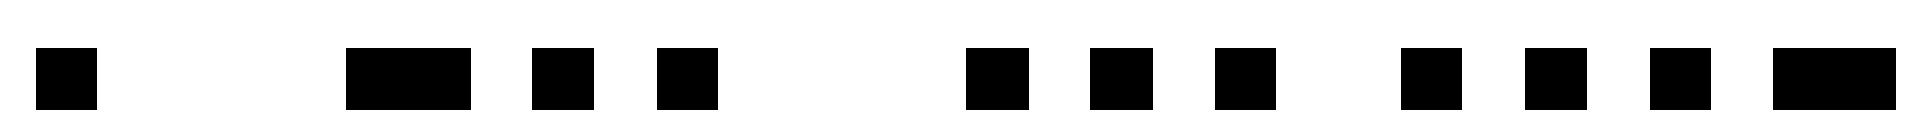
\includegraphics[width=\columnwidth]{background/temporal_parity-10-200-3-input.pdf}
  }

  \subfloat[Correct output]{
    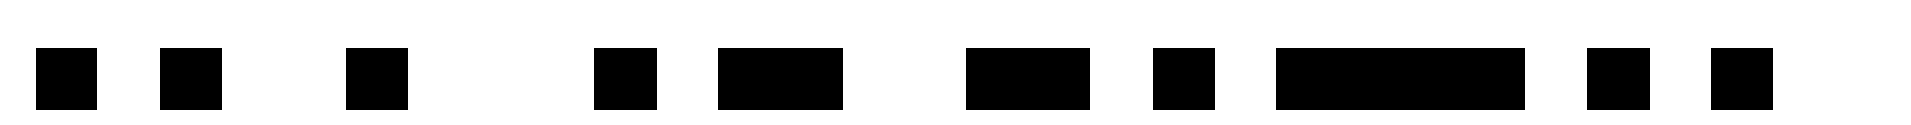
\includegraphics[width=\columnwidth]{background/temporal_parity-10-200-3-output.pdf}
  }

  \caption{
    The first 30 elements of a Temporal Parity task with $[n=3, t=0]$.
    A one is visualized as white, while a zero is black.
    We see that correct output at time $i$ is equal to there being an odd number of $1$s in inputs $[i, i-1, i-2]$
  }
  \label{figure:temporal-parity}
\end{figure}

\subsection{Computational capability}
\label{section:computational-capability}
For an RBN-reservoir to perform well at computational tasks,
it must be able to both forget past perturbations and keep two input streams that have begun converging separated \cite{bertschinger2004real}.

These two properties are coined \textit{fading memory} and \textit{separation property},
and can be measured \cite{rbn-reservoir} as follows.

Create two equal input streams \#1 and \#2 of length $T$.
If measuring \textit{fading memory}, flip the first bit in stream \#2.
If measuring \textit{separation property}, flip all bits up to bit $T-t$ in stream \#2
($t$ being the required depth of separation).
For both input streams, reset reservoir state, perturb the reservoir with the input stream,
and store the final state.
The score of the measure is then defined as the normalized hamming distance between the resulting states.
The computational capability $\Delta$ of an RBN-reservoir is then defined as
\begin{equation}
  \Delta_{Tt} = separation\_property_{Tt} - fading\_memory_{T}
\label{formula:accuracy}
\end{equation}
Analyzing different RBN-reservoirs with this metric \cite{rbn-reservoir},
a high $\Delta$ is found to correlate with critical connectivity ($\langle K \rangle = 2$).
For all RBN-reservoirs, $\Delta$ drops when increasing the required separation $t$,
and is maximized when one doesn't have to remember anything at all ($t=0$).

\subsection{Optimal perturbance}
\label{section:optimal-perturbance}
It is found that the optimal amount of reservoir perturbance,
adjustable by the number of connections between the input layer and the reservoir,
depends on both the task size, how many steps in time are required to be remembered,
and the dynamics of the reservoir.
\textit{Chaotic reservoirs} require few input connections to be able to properly spread information,
but perform poorly on larger tasks due to past perturbations still floating around the reservoir.
\textit{Ordered reservoirs} quickly forget past perturbations, allowing some success for larger tasks,
but their inability to remember past perturbations renders them useless for many tasks.
\textit{Critical reservoirs} require connectivity somewhere in the middle.
Able to forget as well as remember, they perform accurately independent of task size.

\section{Evo Materio}
\todo{Gotta write about Evo Materio}

\section{Results from my forprosjekt}
\todo{Gotta present results from my forprosjekt}

\section{Write about the bucket of water}
\todo{Gotta write about the bucket of water}

\cleardoublepage
